
\chapter{Arbeitsablauf}
\label{cha:Arbeit}
\todo{Register beschreiben!}
\begin{Tipp}
Die Schritte in diesem Kapitel folgen dem chronologischen Aufbau des Projektes.
\end{Tipp}
Das Kapitel \ref{sec:Erste_Schritte} dient dazu den Mikrocontroller so zu programmieren, dass die notwendigen Grundvoraussetzungen für dieses Projekt geschaffen werden. Diese Programmierung lässt sich am einfachsten in einer Entwicklungsumgebung(siehe Kapitel \ref{sec:Entwicklungsumgebung}) schreiben. Das Ziel des Programms besteht darin Spannungen an den Pins des Mikrocontrollers auszugeben oder auszuwerten und somit Komponenten wie LEDs, LC-Display, Taster und serielle Schnittstellen anzusteuern.\\
Das Kapitel \ref{sec:Protokolle} beschreibt die Arbeitsschritte zur Erarbeitung der Protokolle die zur Kommunikation zwischen dem PC und den Peripheriegeräten notwendig sind.\\
Im Kapitel \ref{sec:Komm_SM} geht es um die Kommunikation mit der Schrittmotorkarte.\\
In den Arbeitsschritten in Kapitel \ref{sec:Verbesserung_Hardware} geht es um die Entwicklung und Verbesserung von Hardware. 
Diese wird so erweitert, dass sie den Vorgaben entspricht.\\
In den Arbeitsschritten \ref{sec:Komm_RF2004} wird beschrieben wie die Software so erweitert wird, dass auch sie allen Vorgaben genügt.\\

Im letzten Arbeitsschritt \ref{...} wird dann noch die Entwicklung des Platinenlayouts und des Einschubes erklärt.
\todo{Umstellungsprobleme}
\section{Bereitstellen grundlegender Funktionalitäten}
\label{sec:Erste_Schritte}
Im ersten Schritt ging es darum, den Drehtisch mithilfe eines Mikrocontrollers um 90° zu drehen.\\
Der Mikrocontroller befindet sich auf dem STK 500(siehe Kapitel \ref{sec:STK500}). Dieses bietet grundlegenden Funktionalitäten wie Taster, LEDs, eine Programmierschnittstelle und eine serielle Schnittstelle.
Um die Komponenten sinnvoll im Mikrocontroller nutzen zu können müssen dafür Funktionalitäten wie z.B. Bibliotheken bereit gestellt werden oder Register initialisiert werden.\\
Die folgenden Kapitel beschreiben dieses Bereitstellen der Funktionalitäten.

\begin{Tipp}
Die Codelistings in diesem Kapitel sind thematisch zusammen gefasst und gekürzt um die Lesbarkeit
und das Verständnis zu gewährleisten. Ein komplettes Codelisting des Hauptprogramms befindet
sich im Anhang \ref{cha:CodeComplete}. Der komplette Code, mit allen Bibliotheken, liegt dem Praxisbericht
als CD oder Archiv bei.
\end{Tipp}

\subsection{Taster nutzbar machen}
\label{sec:Taster}
Um die Taster des STK500 im Mikrocontroller nutzen zu können müssen diese entprellt werden.\\
Im ersten Schritt verband ich die Stiftleiste des PortA mit der Stiftleiste für die Taster.\\
Das Entprellen der Taster realisierte ich softwareseitig in dem ich die Bibliothek \cite{uC:Dannegger} von Peter Dannegger einband.\\
Diese habe ich heruntergeladen und in das Projektverzeichnis entpackt.\\
Mit Zeile 1 des Codelisting\ref{lst:Taster} wird die Bibliothek in das Programm eingebunden. Die Zeilen 3-10 spiegeln die Funktion zum Initialisieren der Bibliothek wieder.\\
Nach dem Einbinden der Bibliothek war es möglich Funktionen wie z.B. get\_key\_press() zu nutzen um den Status der Taster prellfrei auszulesen und diese Information für Entscheidungen im Programm zu verwenden. 

\lstset{language=C, basicstyle=\footnotesize, showstringspaces=false, tabsize=8}
\lstinputlisting[label=lst:Taster,caption=Taster]{Code/taster.txt}

\subsection{LEDs ansteuern}
\label{sec:LED}
Die LEDs sollen im Programmablauf nutzbar sein.\\
Dazu verband ich zuerst die Stiftleiste von \emph{PortB} mit der LED Stiftleiste.\\
Um LEDs an \emph{PortB} betreiben zu können musste ich die Pins im \Fachbegriff{Register} \emph{DDRB} als Ausgänge definieren. Dies geschieht in Zeile 3 des Codelisting \ref{lst:LED}. Die Bibliothek zum Entprellen der Taster nutzte die Variablen \emph{LED\_DDR} und \emph{LED\_PORT}. Auch ich nutzte diese Variablen um auf die Register zuzugreifen, da dies eine bessere Übersicht gewährleistet.\\
Die Werte im 8-Bit Register \emph{LED\_PORT} spiegeln die Spannungen an den Pins des \emph{PortB} am Mikrocontroller wieder.\\
Da die LEDs auf dem STK500 mit \Fachbegriff{active-low-Logik} betrieben werden, muss das jeweilige Bit gelöscht, also auf ''0'', gesetzt werden damit die LED leuchtet.
Um alle Bits in einem Register zu verändern kann das Register mit einem 2-stelligen Hex-Wert(8-Bit) beschrieben werden. In Zeile 4 werden so alle Bits auf ''1'' gesetzt.\\
Um ein einzelnes Bit zu verändern, können die Zeilen 5 und 6 verwendet werden. Dabei steht das x in \emph{PBX} für die x-te Stelle im Register die gesetzt oder gelöscht werden soll.\\
Es ist damit möglich im Programmablauf einzelne LEDs anzusteuern.

\lstset{language=C, basicstyle=\footnotesize, showstringspaces=false, tabsize=8}
\lstinputlisting[label=lst:LED,caption=LEDs]{Code/led.c}

\subsection{LCD ansteuern}
\label{sec:LCD}
Um den aktuellen Status des Motor komfortabel anzeigen zu können und den Mikrocontroller "Menü basiert" steuern zu können verwendete ich ein LC-Display.\\
Die meisten LC-Displays werden auf die selbe Art angesteuert. Hier gibt es fertige Bibliotheken die frei genutzt werden können. Im Projekt entschied ich mich für die von Peter Fleury\cite{uC:Fleury}.\\
Dazu lud ich die Bibliothek herunter und entpackte die Dateien \emph{lcd.c} und \emph{lcd.h} in das Projektverzeichnis. \\
Die Bibliothek wird mit \#include ''lcd.h'' eingebunden.\\
In der \emph{lcd.h} mussten noch die Daten des Displays eingegeben werden(siehe Codelisting \ref{lst:LCD}).
Danach kann das Display mit den Befehlen aus Zeile 11--20 angesteuert werden.

\lstset{language=C, basicstyle=\footnotesize, showstringspaces=false, tabsize=8}
\lstinputlisting[label=lst:LCD, caption=lcd.h (Auszug)]{Code/lcd_def.txt}

\subsection{Serielle Schnittstelle ansteuern}
\label{sec:RS232}	
\Fachbegriff{RS-232} ist der Name der am meisten verwendeten seriellen asynchronen Schnittstelle, im Fachjargon auch Übertragungsstandard genannt, um Daten zwischen zwei elektronischen Geräten hin und her zu schicken (im Fachjargon: Datenkommunikation). \cite{uC:RS232}\\
Auf dem STK500 ist bereits eine serielle Schnittstelle vorbereitet. Um diese nutzen zu können musste ich den ersten UART des Mikrocontrollers(PortC 3:4) mit der Stiftleiste Rx/Tx auf dem STK500 verbinden.\\
Eine weitere Schnittstelle baute ich auf einem Steckbrett auf. Diese verband ich mit dem zweiten UART des Mikrocontrollers(PortC 1:2).\\
Um die Schnittstellen im Mikrocontroller nutzen zu können musste ich diese auch noch in der Software vorbereiten.\\
Das Codelisting \ref{lst:RS232} teilt sich in 4 wesentliche Bereiche: \\
\begin{itemize}
\item Zeilen 1 -- 2: Setzen der Baudrate und einbinden der benötigten Bibliotheken.
\item Zeilen 4 -- 16: Initialisieren der Schnittstellen durch setzen der richtigen Bits in den entsprechenden Registern.
\item Zeilen 17 -- 32: Funktionen zum Senden von Daten
\item Zeilen 34 -- 65: Funktionen zum Empfangen von Daten
\end{itemize}
\lstset{language=C, basicstyle=\footnotesize, showstringspaces=false, tabsize=8}
\lstinputlisting[label=lst:RS232,caption=RS-232]{Code/rs232.txt}
Mir stehen dadurch die essentiellen Funktionen \emph{uart\_put\_string()} und \emph{uart\_get\_string()} zur Verfügung. Mit diesen kann der Mikrocontroller über die serielle Schnittstelle Strings senden und empfangen.


\section{Protokolle als notwendige Vorrausetzung zur Kommunikation zwischen PC und Peripheriegeräten} 
\label{sec:Protokolle}
Das Ziel das erreicht werden sollte, bestand darin, dass der PC mit den Peripheriegeräten und die Peripheriegeräte untereinander miteinander kommunizieren sollten.\\
Die Befehlssätze die im Projekt verwendet werden um mit den Schrittmotorsteuerungen zu kommunizieren, werden als Protokolle bezeichnet. In diesen Protokollen ist geregelt, welche Befehle ausgesendet werden müssen und welche Antworten auf diese Befehle erwartet werden.\\
Jede Schrittmotorkarte verwendete ein eigenes Protokoll.
Die Software RapidForm2004 kannte mehrere Protokolle um Schrittmotorkarten anzusteuern. Die vorhandenen Schrittmotorkarten hatten jedoch ein eigenes Protokoll das nicht in RapidForm2004 vorhanden war.\\
Nun soll auch der Mikrocontroller mit RapidForm2004 und einer der vorhandenen Schrittmotorkarten kommunizieren. 
Dazu musste der Mikrocontroller zumindest eines der Protokolle aus RapidForm2004 kennen und das Protokoll der vorhanden Schrittmotorkarten.\\
In der ersten Phase verwendete ich die Software \emph{Free Serial Port Monitor} um die Kommunikation zwischen dem PC und den Peripheriegeräten abzuhören. Dies hatte jedoch den Nachteil, das RapidForm2004 erst den nächsten Befehl sendete, wenn der erste mit der erwarteten Antwort quittiert wurde. Die Befehle die RapidForm erwartete, konnten zwar teilweise aus den Betriebsanleitungen der Schrittmotoren entnommen werden, dies war jedoch sehr mühsam.\\
Nach einiger Zeit kam ich auf die Idee \Fachbegriff{Reverse-Engineering} zu verwenden und war dadurch in der Lage alle Protokolle aus der ausführbaren Datei von RapidForm2004 auszulesen.\\
Das Codelisting \ref{lst:Proto_RF_Zeta} zeigt einen Auszug für das Protokoll eines Zeta Schrittmotors. Im Anhang befinden sich alle Protokolle.
\lstset{language=C, basicstyle=\footnotesize, showstringspaces=false, tabsize=8}
\lstinputlisting[label=lst:Proto_RF_Zeta,caption=Protokoll aus Rapidform: Zeta]{Code/Protokolle_RF_Zeta.txt}
Somit standen mir die Protokolle aller Schrittmotorsteuerungen zur Verfügung. Diese speicherte ich in einer Textdatei ab um sie bei Bedarf im Mikrocontroller Programm zu verwenden. Das bedeutete, dass nun alle Befehlssätze und deren Antworten, die ich im Projekt verwenden würde, vorhanden waren.

\section{Kommunikation mit der Schrittmotorsteuerung}
\label{sec:Komm_SM}
\subsection{Befehle senden}
\label{sec:menu}
Im nächsten Schritt ging es darum, Befehle an die Schrittmotorkarte zu versenden. Da es nicht möglich war, für jeden Befehl eine eigene Taste zu verwenden, 
entschied ich mich für eine Menü basierte Steuerung auf dem LC-Display. Im Menü lies sich mit den Tasten \emph{Hoch} \emph{Runter} \emph{Ok} und \emph{Zurück} navigieren.\\
Ich passte die Menüstruktur meinen Bedürfnissen an. Dazu gehörte, dem Menü die Befehle und die Funktion zum Versenden von Befehlen bekannt zu machen.
Außerdem musste der Menü-Bibliothek die Befehle der LCD-Bibliothek bekannt gemacht werden.\\
Die Zeilen 1--6 des Codelisting \ref{lst:Menu} dienen zum Einbinden der benötigten Bibliotheken.\\
Die Zeilen 8-16 zeigen eine vereinfachte Struktur meines  Hauptprogramms. Wird ein Taster gedrückt wird dies durch die get\_key\_press() Funktion, bekannt aus Kapitel \ref{sec:Taster}, erkannt und die entsprechende Menü Funktion aufgerufen.
\lstset{language=C, basicstyle=\footnotesize, showstringspaces=false, tabsize=8}
\lstinputlisting[label=lst:Menu,caption=Menü]{Code/menu.c}
Wird einer der Menüpunkte aufgerufen, wird die im Menüpunkt hinterlegte Funktion mit dem hinterlegten Parameter aufgerufen.
Wird beispielsweise der Befehl \emph{+90} ausgewählt, wird die hinterlegte Funktion \emph{menu\_puts()}(Codelisting \ref{lst:Menu} Zeile 18-28) mit dem hinterlegten Wert aufgerufen. Diese sendet dann mit der aus Kapitel \ref{sec:RS232} bekannten Funktion \emph{uart\_puts(arg, dir)} einen Befehl an die Schrittmotorsteuerung.\\
Nun kann mit den Tasten Hoch, Runter, Ok und Zurück im Menü Navigiert werden. Ist ein Befehl ausgewählt kann dieser durch Drücken des Ok Knopfes ausgewählt werden. Wird z.B. der Menüpunkt \emph{+90} ausgewählt wird die Zeichenkette ''M 125000'' an die Drehtischsteuerung gesendet. Der Drehtisch dreht sich um 90° gegen den Uhrzeigersinn.
\todo{Zukunft: Einstellbarer Winkel}
\lstset{language=C, basicstyle=\footnotesize, showstringspaces=false, tabsize=8}
\lstinputlisting[label=lst:Menu_Baum,caption=Menü Baum]{Code/menu_main.txt}
\subsection{Antworten Empfangen und speichern}
\label{sec:Empfangen_Schrittmotor}
In diesem Arbeitsschritt stellte ich die Funktionalität zum Empfangen von Antworten der Schrittmotorsteuerung auf Befehle des Mikrocontrollers her. Diese Antworten sollten gespeichert und an eine Auswerte-Funktion weiter gegeben werden.\\
Dazu lies ich in der Hauptschleife des Programms ständig das Eingangsregister der ersten seriellen Schnittstelle abfragen(siehe Codelisting \ref{lst:rs232empfang} Zeile 10--13). Dieses Vorgehen bezeichnet man als \Fachbegriff{Polling}.
Sind Daten im Register vorhanden, wird \emph{LED3} eingeschaltet und die Funktion \emph{uart\_rx(int dir)} mit dem Parameter \emph{D\_Stepper} aufgerufen. Dieser Parameter gibt an das der Befehl von der, für die Schrittmotorkarte zuständigen seriellen Schnittstelle empfangen wurde. Dadurch wird bestimmt, dass der empfangene \Fachbegriff{String} aus dem richtigen Datenempfangsregister ausgelesen wird und wie er weiterverarbeitet wird.\\
Die Funktion \emph{uart\_rx(dir)} liest dann das Empfangsregister mit der aus Kapitel \ref{sec:RS232} bekannten Funktion \emph{uart\_get\_string(str\_rx, dir)} aus und schreibt den empfangenen String in die Variable \emph{str\_rx}(Codelisting \ref{lst:rs232empfangstepper}, Zeile 7).\\
In einer if-Abfrage wird entschieden, von welcher Schnittstelle der empfangene Befehl kam. Da \emph{D\_Stepper} übergeben wurde, wird der if-Teil der Abfrage ausgeführt.\\
In dieser wird der empfangene String an die Auswerte-Funktion  für die Schrittmotorkarte(Codelisting \ref{lst:rs232empfangstepper}, Zeile 15-45) übergeben.
Durch diesen Teil des Programms ist es nun möglich Antworten der Schrittmotorkarte zu empfangen, zu speichern und an die  Auswerte-Funktion für die Schrittmotorkarte zu übergeben.
\lstset{language=C, basicstyle=\footnotesize, showstringspaces=false, tabsize=8}
\lstinputlisting[label=lst:rs232empfangstepper, caption=RS-232 Empfang]{Code/rs232_empfang_stepper.c}


\subsection{Antworten auswerten}
\label{sec:Auswerten}
Die Funktion zum Auswerten empfangener Strings spielt eine zentrale Rolle im Projekt. Diese Funktion soll es ermöglichen, ankommende Strings im Mikrocontroller gegen den Antwortsatz aus den Protokollen zu prüfen und eine entsprechende Reaktion auszuführen.\\
In der Auswerte-Funktion wird der übergebene String mittels der Funktion \emph{FindStringInArray(str\_rx, pOptions, 1)}(Codelisting \ref{lst:FindString}) gegen ein Array(Codelisting \ref{sec:switchStepper}, Zeile 2) mit vorhanden Befehlen geprüft. Ist der String in diesem Array vorhanden wird die Position des Strings im Array zurückgegeben. Ansonsten "99".\\
In einer anschließenden switch/case-Struktur wird dann anhand der Position das Verhalten des Mikrocontrollers festgelegt.\\
Wird beispielsweise der String \emph{\#} empfangen, wird Position \emph{0} zurück gegeben und auf dem Display wird \emph{Erfolgreich} ausgegeben.\\
Durch diese Funktion kann nun auf Strings reagiert werden und eine entsprechende Reaktion seitens des Mikrocontrollers erfolgen.
\lstset{language=Java, basicstyle=\footnotesize, showstringspaces=false, tabsize=8}
\lstinputlisting[label=lst:FindString, caption=FindStringInArray()]{Code/FindString.c}
\lstset{language=Java, basicstyle=\footnotesize, showstringspaces=false, tabsize=8}
\lstinputlisting[label=lst:switchStepper, caption=switchStepper()]{Code/switch_stepper.c}

\section{Verbesserungen an der vorhandenen Hardware}
\label{sec:Verbesserung_Hardware}
\subsection{Netzteil modular erweiterbar machen}
\label{sec:Netzteil}
Ziel dieses Arbeitsschrittes war es die festen Lötverbindungen zwischen dem PC-Netzteil und den einzelnen Karten im 19''-Rack durch Steckverbindungen zu ersetzen und dadurch leicht erweiterbar zu machen.\\
Ich ersetzte die festen Lötverbindungen der Schrittmotorkarten  durch Standard PC-Netzteil Stecker. Nun versah ich auch den Einschub für die Mikrocontroller-Platine mit einem Standard PC-Netzteil Stecker. Die Mikrocontroller-Platine speiste ich mit 5V.
Die \Fachbegriff{Logikbausteine} der Schrittmotorkarten wurden ebenfalls mit 5V gespeist. Die Schrittmotoren wurden über die Schrittmotorkarten mit 12V gespeist.\\
Diese Stecker ließen sich nun einfach mit den Buchsen des Netzteils verbinden. Mittels eines Y-Kabels(siehe Abbildung \ref{fig:Y-Kabel}) konnte ich nun leicht weitere Buchsen hinzufügen.\\
Dadurch konnte das Netzteil nun einfach ein- und ausgebaut werden, bzw. das System leicht mit neuen Einschubkarten erweitert werden.
\begin{figure}[h]
\centering
\includegraphics[width=100pt]{Y-Kabel.jpg}
\caption{Stromverbinder - Y-Kabel\cite{kosatec}}
\label{fig:Y-Kabel}
\end{figure}
\todo{\url{http://www.kosatec.de/prod_images/kc/640x480/100539.jpg}}

\subsection{Inbetriebnahme der zweiten Schrittmotorkarte}
Zu Anfang stand mir nur eine Schrittmotorkarte für die Rotation des Drehtisches zur Verfügung. Mit einem zweiten Schrittmotor konnte der Tisch in der Höhe verstellt werden. Hierzu fehlte aber noch eine zweite Schrittmotorkarte. Diese musste noch vorbereitet und mit der ersten verbunden werden.\\
Dazu bereitete ich, wie in Kapitel \ref{sec:Netzteil} beschrieben, einen weiteren Einschubplatz für die Schrittmotorkarte vor. Ich versah die Karte mit einer Frontblende und brachte auf dieser eine Buchse für die Motorverkabelung und je eine Buchse und einen Stecker für die seriellen Schnittstellen an. Diese verlötete ich mit den entsprechenden Anschlüssen auf der Schrittmotorkarte. Ich schob die Karte in den Einschubplatz und verband diese als \Fachbegriff{Daisy-Chain} mit der ersten Schrittmotorkarte. Dadurch konnte die zweite Schrittmotorkarte über die erste angesteuert werden.\\
Somit stand mir eine Baugleiche Schrittmotorkarte zur Verfügung. Nun  konnte ich den Schrittmotor für die Höhenverstellung ansteuern. 

\subsection{Motor- und Endschalterverkabelung}
Zwischen der zweiten Schrittmotorkarte und dem zugehörigen Schrittmotor, der für die Höhenverstellung zuständig ist, war noch kein Kabel vorhanden. Dieses musste noch gefertigt und um 3 Leitungen für die Endschalter erweitert werden.\\
Dafür besorgte ich in der Werkstatt ein 7 adriges Kabel(Abbildung \ref{fig:Motorverkabelung}) und lies die passenden Endstecker bestellen. Die Belegung wählte ich gleich zum Kabel für den ersten Schrittmotor, erweiterte sie jedoch um die 3 Adern für die beiden Endschalter. Tabelle \ref{tab:Motorverkabelung} gibt die Belegung des Kabels wieder.\\
Somit stand ein Kabel zur Verfügung mit dem sowohl der Schrittmotor gesteuert, als auch der Status der Endschalter ausgelesen werden konnte.
\todo{Belegung überprüfen!}
\begin{figure}[h]
\centering
\includegraphics[width=\textwidth]{Kabel.pdf}
\caption{Motor- und Endschalterverkabelung}
\label{fig:Motorverkabelung}
\end{figure}
\begin{longtable}{|c|l|} 
\caption{Motor- und Endschalterverkabelung} \\
\hline
\label{tab:Motorverkabelung}
1 & Phase A \\ 
\hline 
2 & Phase B \\ 
\hline 
3 & Phase C \\ 
\hline 
4 & Phase D \\ 
\hline 
5 & Endschalter oben \\ 
\hline 
6 & Endschalter unten \\ 
\hline 
7 & Endschalter Masse \\ 
\hline 
\end{longtable} 

\subsection{Inbetriebnahme der induktiven Endschalter}
Nun ging es darum, die vorgegeben induktiven Endschalter mit der Schrittmotorkarte und dem Mikrocontroller zu verbinden. Dadurch sollte gewährleistet sein, dass der Drehtisch nicht über den Arbeitsbereich hinaus bewegt wird. Zusätzlich sollte das Erreichen der Endpositionen auf dem LC-Display angezeigt werden.\\
Da die Schrittmotorkarte nur mechanische Endschalter unterstützt, ließen sich die induktiven Endschalter nicht ohne weiteres nutzen. Um die induktiven Endschalter nutzen zu können, musste die Spannung über einen Spannungsteiler heruntergesetzt werden. Ich umging die standardmäßigen Eingänge für die mechanischen Endschalter und schloss die induktiven Endschalter direkt an den Optokoppler an, welcher für die mechanischen Endschalter zuständig war. Dadurch wurden die Signale der Endschalter für die Schrittmotorkarte nutzbar. 
\begin{figure}[h]
\centering
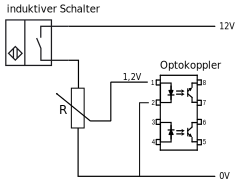
\includegraphics{Endschalter.pdf}
\caption{Motor- und Endschalterverkabelung}
\label{fig:Motorverkabelung}
\end{figure}
Ein weiteres Problem bestand darin, dass, wenn der Tisch sich bereits in der Endposition befand, die Endschalter noch nicht aktiviert wurden. Dies lag daran, dass der Metallstutzen, der die Endschalter auslösen sollte, sich nicht im Schaltbereich der induktiven Schalter befand. Zur Abhilfe lies ich einen längeren Metallstutzen von der Werkstatt anfertigen.\\
Wenn der Tisch sich in der Endposition befindet, sollte dies auch auf dem LC-Display der Mikrocontroller-Platine angezeigt werden. Die Signale der Endschalter liegen auf der Rückseite der Schrittmotorkarte am Verbindungsstecker an. Ich lötete eine Brücke zwischen den Verbindungssteckern der Schrittmotorkarte und des Mikrocontrollers.\\
Auf der Mikrocontroller-Platine sind diese beiden Pins mit je einem Pin des Mikrocontrollers verbunden. Diese beiden Pins werden im Mikrocontroller als \Fachbegriff{Interrupts} definiert. Die Interrupt-Service-Routine zum Anzeigen der Nachricht auf dem LC-Display wird in Kapitel \ref{sec:Endschalter_SW} beschrieben.\\
Da die Signale der Endschalter nun an der Schrittmotorkarte anlagen, konnte diese den Motor stoppen wenn die Endschalterpositionen erreicht werden. Zusätzlich lagen die Signale am Mikrocontroller an. Dieser konnte dadurch auf dem Display die Meldung \emph{Endschalterposition erreicht!} ausgeben.

\subsection{Zweite serielle Schnittstelle}
Das STK500 bot nur eine serielle Schnittstelle. Um zusätzlich zur Schrittmotorkarte auch mit dem Erfassungs-PC kommunizieren zu können benötigte ich eine zweite serielle Schnittstelle.\\
Dafür baute ich auf einem Steckbrett eine zweite serielle Schnittstelle nach dem Schaltplan in Abbildung \ref{fig:MAX232} auf.\\
Dadurch war es mir möglich über zwei seriellen Schnittstellen gleichzeitig zu kommunizieren.
\begin{figure}[h]
\centering
\includegraphics[width=0.6\textwidth]{AVR-RS232}
\caption{Schema: MAX232}
\label{fig:MAX232}
\citep{uC:RS232}
\end{figure}

\section{Kommunikation mit RapidForm2004}
\label{sec:Komm_RF2004}
RapidForm2004 sendet Befehle die für die Drehtischstuerung bestimmt sind an den Mikrocontroller. Diese sollen dort empfangen, ausgewertet und in verständlicher Form an die Drehtischsteuerung weiter gegeben werden. RapidForm2004 verwendet dabei verschiedene Protokolle für verschiedene Schrittmotorsteuerungen. Für jedes dieser Protokolle schrieb ich eine eigene Auswerte-Funktion. Im folgenden Kapitel wird nun das Empfangen der Befehle beschrieben und eine erste Auswertung die den empfangenden Befehl dem Protokoll einer Schrittmotorsteuerung zu ordnet.\\
Nach der Beschreibung der Auswerte-Funktionen sollte der Befehl an die Drehtischsteuerung gesendet und die Antwort der Drehtischsteuerung ausgewertet werden.
Abschließend sollte eine entsprechende Antwort an RapidForm2004 zurück gesendet werden. \\
Die Kommunikation mit RapidForm2004 ist sehr ähnlich zu der mit der Schrittmotorsteuerung. Diese wurde bereits in Kapitel \ref{sec:Komm_SM} ausführlich beschrieben. 

\subsection{Befehle empfangen}
Zuerst sollten nun Befehle von RapidForm2004 an den Mikrocontroller, gespeichert werden. Anschließend wird die automatische Protokollwahl beschrieben.\\
Um anstehende Befehle zu empfangen verwendete ich, ähnlich wie in Kapitel \ref{sec:Empfangen_Schrittmotor}, eine Funktion die ständig das Eingangsregister der ersten seriellen Schnittstelle abfragte(siehe Codelisting \ref{lst:rs232empfangrf}) Auch hier wurde die Funktion \emph{uart\_rx(dir)} aufgerufen, jedoch mit dem Parameter \emph{D\_RapidForm}. Der empfangenen String wurde auch hier in die Variable \emph{str\_rx} gespeichert.\\
Somit konnten nun auch Strings von RapidForm2004 empfangen werden.
\lstset{language=Java, basicstyle=\footnotesize, showstringspaces=false, tabsize=8}
\lstinputlisting[label=lst:rs232empfangrf, caption=RS-232 Empfang - RapidForm2004]{Code/rs232_empfang.c}

\subsubsection{Automatische Protokollwahl}
\label{AutoProtokoll}
Nun ging es darum, dass RapidForm2004 anhand eines ersten Befehls der empfangen wurde, festlegt mit welchem Protokoll fortan kommuniziert werden sollte. Dieses Protokoll sollte dann global festgelegt sein und alle weiteren Befehle sollten an die entsprechende Auswerte-Funktion übergeben werden.\\
In der Funktion \emph{uart\_rx()}(Codelisting \ref{lst:uartrx}) wurde nun in der ersten \emph{if-Abfrage} entscheiden, von welcher Schnittstelle der empfangene Befehl kam. Diese verzweigte nun, da \emph{D\_RapidForm} übergeben wurde, in den else-Teil.\\
In diesem überprüfte ich mit mehreren \emph{if-Abfragen}, ob bereits ein Protokoll für einen bestimmten Motor ausgewählt wurde.
War dies nicht der Fall, wurde der String an die Funktion \emph{switch\_Motor()}(Codelisting \ref{lst:switchMotor}) übergeben. Diese prüfte mit der aus Kapitel \ref{sec:Auswerten} bekannten Funktion \emph{FindStringInArray()}, den angekommenen String gegen die Initialisierungsbefehle der einzelnen Protokolle. Die Initialisierungsbefehle sind die ersten Befehle die RapidForm2004 an eine Schrittmotorsteuerung sendet um zu prüfen ob diese vorhanden ist. In diesem ersten Schritt wurde der String nur zur Identifizierung des von RapidForm2004 angefragten Protokolls verwendet. Die Antworten auf diese Strings wird erst in den Nachfolgenden Kapiteln beschrieben.\\
Die Funktion \emph{switch\_Motor()} gab einen numerischen Wert zurück. Jede Zahl entsprach dabei einem Motorprotokoll. Die Zahlenwerte wurden dabei mittels Makro-Definitionen(Codelisting \ref{lst:rs232empfang} Zeile 1-6) mit lesbare Text-Variablen ersetzt. Dies erhöhte die Lesbarkeit und das Verständnis ungemein.\\
War dieser Schritt erfolgreich, wurden in den folgenden if-Abfragen die richtige Auswerte-Funktion aufgerufen. Konnten die Funktion \emph{switch\_Motor()} den empfangen Befehl nicht zuordnen, gab sie \emph{M\_UNK} zurück und es wurde auf dem Display \emph{Unbekannter Motor!} ausgegeben.\\
Somit war es mir möglich Befehle von RapidForm2004 zu empfangen und an eine entsprechende Auswerte-Funktionen zu übergeben. Zusätzlich wurde die Programmierung dadurch wesentlich robuster, da unbekannte Befehle ignoriert wurden.\\
Ein Nachteil dieses Vorgehens besteht darin, dass für eine erneute Protokollwahl der Mikrocontroller neu gestartet werden muss. Ein Beheben dieses Nachteils wäre nicht ohne weiteres möglich gewesen.

\lstset{language=C, basicstyle=\footnotesize, showstringspaces=false, tabsize=8}
\lstinputlisting[label=lst:uartrx,caption=Funktion: uartrx()]{Code/uart_rx.c}

\lstset{language=C, basicstyle=\footnotesize, showstringspaces=false, tabsize=8}
\lstinputlisting[label=lst:switchMotor,caption=Funktion: switchMotor]{Code/switch_Motor.c}

\section{Auswerte-Funktionen}

Die Auswerte-Funktionen sind das Herzstück des Programms. Es ging darum für jedes Protokoll eine eigene Auswerte-Funktion zu schreiben. Diese sollten die von RapidForm2004 kommenden Strings verstehen können und in einen, für die vorhandene Schrittmotorkarte, verständlichen Befehl übersetzen können. Die Funktionen sollten weiterhin prüfen, ob der Befehl von der Schrittmotorkarte erkannt wurde und den Status der Schrittmotorkarte zurück an RapidForm2004 melden.\\


Alle bisherigen Arbeitsschritte hatten zum Ziel die Kommunikation zwischen RapidForm2004 und der ersten Schrittmotorkarte zu ermöglichen. Jetzt fehlte nur noch das Programm zum Übersetzen der Protokolle. 
RapidForm2004 war in der Lage eine Reihe von Befehlen an die Schrittmotorkarte zu senden. Die Schrittmotorkarte konnte die Befehle nicht erkennen, da sie nur ihr eigenes Protokoll verstehen konnte.




Im folgenden Kapitel wird dieser Ablauf nun exemplarisch für das Protokolle eines Isel-Motors erklärt.


Nummer			mWert		c			x			
sz 776			767			363			229
bad 777			22			9872		8
WZ 775			555			6581		178
1. 797			279			8718		11
Kü	774			3			9480		1			



\subsection{Auswerte-Funktion für Isel Motoren}
Nun sollte die Kommunikation zwischen RapidForm2004 und der Schrittmotorkarte beschrieben werden.\\
Wurde wie im Kapitel \ref{sec:AutoProtokoll} beschrieben das Protokoll für einen Isel Motor ausgewählt, wurde der empfangene String, gespeichert in \emph{str\_rx()}, an die Auswerte-Funktion \emph{switch\_Isel(str\_rx)} übergeben. Der Abaluf dieser Funktion ist ähnlich zu dem bei der Kommunikation mit der Schrittmotorkarte(Kapitel \ref{sec:Komm_SM}) und bei der Automatischen Protokollwahl(Kapitel \ref{sec:AutoProtokoll}. In der Funktion hinterlegte ich im Array \emph{pOptions} alle benötigten Befehle des Isel-Protokolls. Mit der aus Kapitel \ref{sec:Auswerten} bekannten Funktion \emph{FindStringInArray(str\_rx, pOptions)} wurde \emph{str\_rx} gegen diese Befehle geprüft. Wurde der Befehl im Array gefunden gab \emph{FindStringInArray} die Position des Strings im Array zurück. Mittels einer \emph{switch-case-Struktur} lies sich nun so für jeden Befehl eine entsprechende Reaktion ausführen. 

\subsubsection{Initialisierung}

\subsubsection{Statusabfrage}
Kommt z.B. der String \emph{@0R} an, wird der Codeblock von \emph{case 4} ausgeführt. Dies ist der Codeblock für eine Statusabfrage. Auf dem LC-Display wird \emph{Satusabfrage:} ausgegeben. Danach wird der entsprechende Befehl für eine Statusabfrage an die Schrittmotorkarte gesendet. Nach einer kurzen Pause von 50ms, um die Verarbeitung auf der Schrittmotorkarte zu gewährleisten, wird mit einer if-Anweisung geprüft ob sich Daten im Schrittmotorkarten seitigen Empfangsregister befinden. Sprich, die Schrittmotorkarte reagiert hat. Ist dies der Fall, wird der Ablauf, bekannt aus Kapitel \ref{sec:Komm_SM}, durchlaufen. Während diesem Ablauf wird die entsprechende Antwort der Schrittmotorkarte auf dem LC-Display ausgegeben. In einer weiteren if-Anweisung wird überprüft ob der angekommene String erfolgreich war. Wenn ja, wird dies an RapidForm2004 gemeldet. Andernfalls zeigt das Display \emph{Fehlgeschlagen} an und sendet eine 1 an RapidForm2004.\\


\subsubsection{Bewegung}

\lstset{language=C, basicstyle=\footnotesize, showstringspaces=false, tabsize=8}
\lstinputlisting[label=lst:switch_Isel,caption=Übersetzungs Logik: Isel]{Code/switch_Isel.txt}


\subsection{Interrupts}
\label{sec:Interrupts}
Viele Mikrocontroller bieten die Möglichkeit Eventbasierte Subroutinen auszuführen. Wenn einer der Interrupts ausgelöst wird, wird das Hauptprogramm unterbrochen und die Entsprechende Interrupt-Service-Routine, kurz ISR, ausgeführt. Nach Beendigung der ISR wird das Hauptprogramm an der  vorherigen Stelle wieder aufgenommen.\\
ISR dürfen nur sehr wenige Befehle enthalten und müssen innerhalb weniger ClockCicles abgeschlossen sein. \\
Interrupts können z.B. der Überlauf eines internen Timer sein, oder ein externens Signal an einem Pin.\\
Im Projekt werden externe Interrupts, Timer-Überlauf Interrupts und der Watchdog Interrupt genutzt. 
\subsubsection{Endschalter}
\label{sec:Endschalter_SW}
Die Endschalter sind über die Schrittmotorkarten und eine Brücke in der Steuerung mit der Mikrocontroller Platine Verbunden. Dort sind sie an 2 Interrupt Pins angeschlossen. \todo{Pins raus suchen!} Bei einem Flanken Wechsel an den Pins wird ein Interrupt ausgelöst. \\
Das Code-Listing \ref{lst:ISR_ES} zeigt die ISR für die Endschalter.
\lstset{language=C, basicstyle=\footnotesize, showstringspaces=false, tabsize=2}
\lstinputlisting[label=lst:ISR_ES,caption=ISR: Endschalter]{Code/ISR_Endschalter.txt}
\subsubsection{Watchdog}
Der \Fachbegriff{Watchdog} ist eine Sicherungseinrichtung des Mikrocontroller. In regelmäßigen Abständen wird überprüft ob das Watchdog Bit gesetzt ist und anschließend zurück gesetzt. Das Bit muss innerhalb der voreingestellten Zeit immer wieder neu gesetzt werden. Dies kann mit der wdt\_reset() Funktion realisiert werden. Ist das Bit nicht gesetzt, wird der Mikrocontroller zurückgesetzt. \todo{Inverse Logik?} Dies geschieht z.B. bei nicht geplanten Endlosschleifen.\\
Wahlweise kann kurz vor dem Reset noch die Watchdog-ISR durchlaufen werden.\\
Im Projekt wird in der ISR die Fehler LED eingeschaltet und eine Meldung auf dem LC-Display ausgegeben. Siehe hierzu auch Listing \ref{lst:Watchdog} Zeilen 12-15.
\lstset{language=C, basicstyle=\footnotesize, showstringspaces=false, tabsize=4}
\lstinputlisting[label=lst:Watchdog,caption=Watchdog]{Code/Watchdog.txt}



\chapter{Probleme und Lösungen}
\section{Entwicklungsumgebungen}
\subsection{AVR Studio 5}
Die von Atmel AVR Studio 5 ist eine von Atmel bereitgestellte Entwicklungsumgebung. Diese scheint jedoch eine fehlerhafte Bibliothek zu enthalten. Die Kombination aus Mikrocontroller ATmega324A und AVR Studio 5 erzeugte nicht nachvollziehbare Probleme. Bei dem selbem Programm und einem anderem Mikrocontroller oder einer anderen Entwicklungsumgebung tauchten keine Fehler auf.
In der Entwicklungsumgebung Eclipse lies sich der Fehler reproduzieren wenn der Pfad der Atmel Bibliotheken eingestellt wurde. Die WinAVR Bibliotheken und eine selbst kompilierte \Fachbegriff{Toolchain} unter Linux zeigten keine Probleme.\\
Daher wechselte ich zur \Fachbegriff{Open Source} Entwicklungsumgebung Eclipse. Erst dadurch wurde es möglich erfolgreich zu arbeiten. Außerdem wurde das Projekt dadurch plattformunabhänig und ich nutzte bis auf RapidForm2004 nur noch freie Open Source Software.\\
\subsection{Eclipse}
Eclipse ist eine in Java programmierte freie Open Source Entwicklungsumgebung für Java. Sie lässt sich durch \Fachbegriff{Plugins} leicht für viele Sprachen erweitern.\\
Mit dem CDT-Plugin, dem AVR-Plugin und einer Bibliothek wie z.B. WinAVR für Windows ist Eclipse eine vollwertige Entwicklungsumgebung für Atmel Mikrocontroller. 
Ergänzt wird diese durch die Programmiersoftware AVR-Dude.\\




\section{Fuses}
\label{sec:Fuses}
Als Fuses werden Register bezeichnet mit denen sich, auf Hardwareebene, das Verhalten des Mikrocontrollers verändern lässt. \\
Im Projekt wurden folgende Fuses problematisch.
\begin{itemize}
\item \textbf{JTAGEN} - Ist dieses \Fachbegriff{Fusebit} gesetzt, werden 4 Pins des PortB genutzt um den Mikrocontroller zu debuggen und können nicht anders genutzt werden. Hardware Debugging bietet viele Vorteile. Diese wurden im Projekt jedoch nicht genutzt da PortB für die LEDs genutzt wurde.
\item \textbf{WDTON} - Ist dieses Fusebit gesetzt läuft der Watchdog Timer immer mit. Wird der Watchdog dann nicht regelmäßig zurückgesetzt startet der Mikrocontroller ständig neu.
\item \textbf{CKDIV8} - Teilt den Systemtakt des Mikrocontroller durch 8. Dies ist Energiesparender. Der geringere Takt muss in F\_CPU angepasst werden da sonst zeitkritische Prozesse mit der falschen Geschwindigkeit ablaufen.
\item \textbf{CKOUT} - An PortB wird an einem Pin der Systemtakt ausgegeben. Dieser kann dann leicht mit einem Frequenz-Messgerät überprüft werden. Der Pin kann dann jedoch nicht anderweitig genutzt werden.
\item \textbf{CKSELX} - Über diese 4 Bits kann der Systemtakt eingestellt werden.
\end{itemize}
\begin{longtable}{|c|l|} 
\caption{Fuses} \\
\hline
\label{tab:Fuses}
OCDEN & On Chip Debugging \\ \hline 
JTAGEN & Hardware Debugging \\ \hline 
SPIEN & Serial Program and Data Downloading \\ \hline 
WDTON & Watchdot Timer always on \\ \hline 
EESAVE & EEPROM memory is preserved through the Chip Erase \\ \hline 
BOOTSZ1 & Select Boot Size \\ \hline 
BOOTSZ0 & Select Boot Size \\ \hline 
BOOTRST & Select Reset Vector \\ \hline 
CKDIV8 & Divide clock by 8 \\ \hline 
CKOUT & Clock output \\ \hline 
SUT1 & Select start-up time \\ \hline 
SUT0 & Select start-up time \\ \hline 
CKSEL3 & Select Clock source \\ \hline 
CKSEL2 & Select Clock source \\ \hline 
CKSEL1 & Select Clock source \\ \hline 
CKSEL0 & Select Clock source \\ \hline 
\end{longtable} 


\section{Platinenlayout}
%Für den Mikrocontroller und seine Peripherie entwickelte ich ein Platinenlayout in der Open Source Software KiCad. \\ 
%Dazu wurden die Schaltungen wie auf dem STK500 in den Schaltplan übernommen und dort das Layout entwickelt. 
%\begin{figure}[htb]
%\centering
%\includegraphics[width=\textwidth]{Translator_white}
%\caption{Platinenlayout}
%\label{fig:Platine}
%\end{figure}
%\todo{Schaltplan und einbinden.}
%\section{19''-Einschub}
%Die Platine für den Mikrocontroller konstruierte ich als 19''-Einschub. Über den rückwärtigen Steckverbinder verband ich die Platine mit der Spannungsversorgung. Zusätzlich kommen hier auch die Signale der Endschalter an.
%An der Vorderseite befestigte ich eine Blende. Auf der Blende befinden sich das LC-Display, fünf Taster, 5 LEDs und 2 serielle Schnittstellen. Alle Bauteile sind steckbar mit der Platine verbunden. \todo{Bild des Einschub}